\documentclass{standalone}
\usepackage{tikz}
\usetikzlibrary{patterns, positioning}

\begin{document}
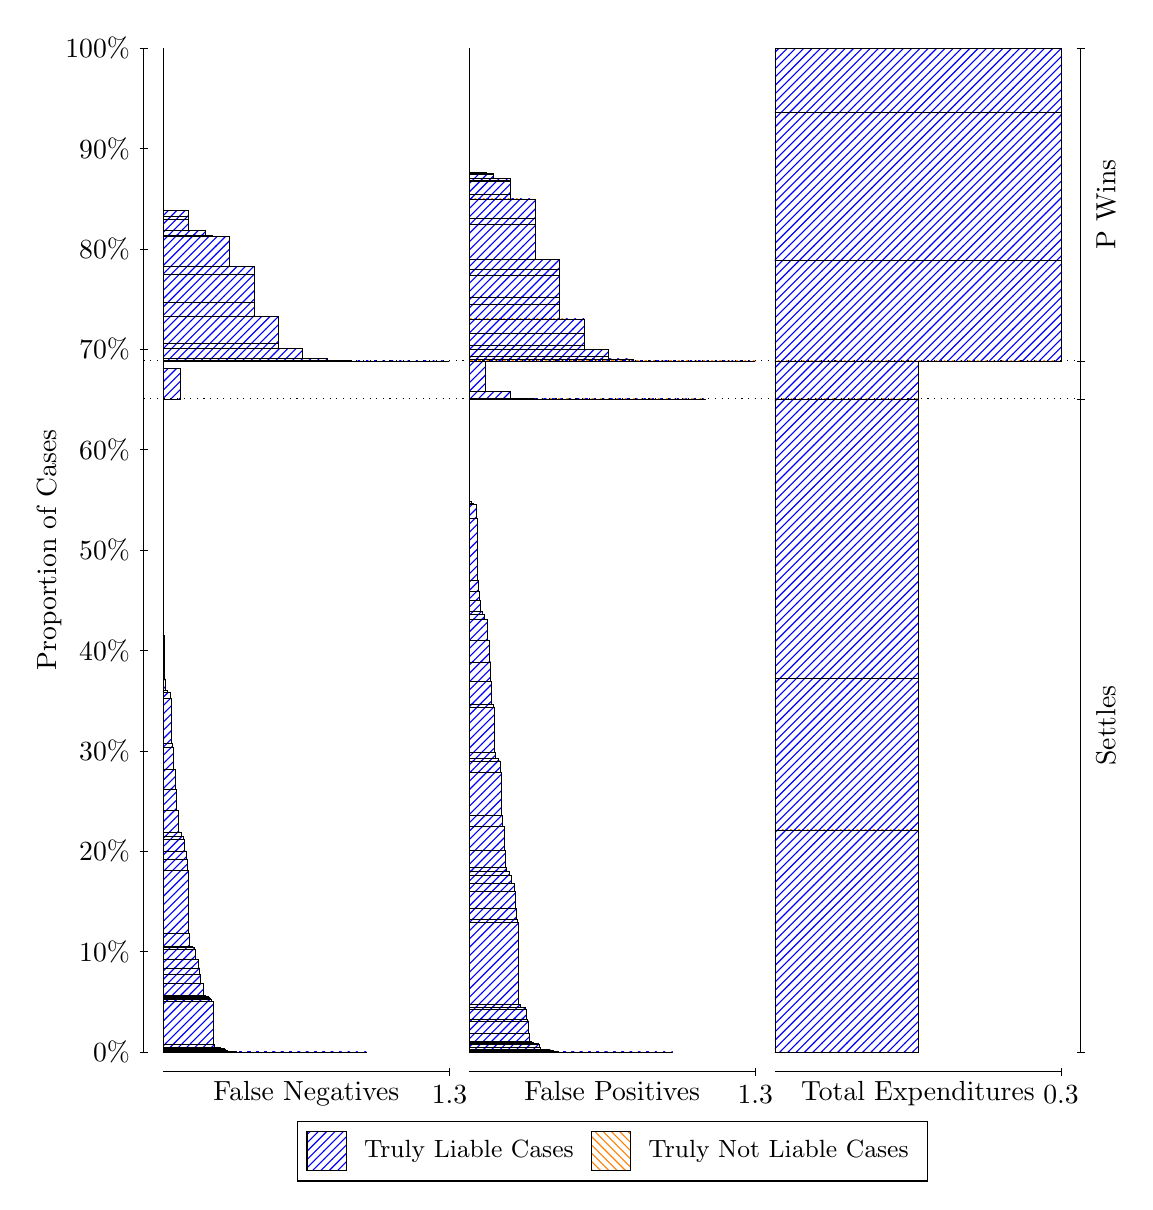
\begin{tikzpicture}
\draw[black, very thin] (1.5,1.75) -- (1.5,14.5);
\node[rotate=90, anchor=center] at (0.3, 8.125) {Proportion of Cases};
\draw[black, very thin] (1.45,1.75) -- (1.55,1.75);
\node[anchor=east] at (1.45, 1.75) {0\%};
\draw[black, very thin] (1.45,3.025) -- (1.55,3.025);
\node[anchor=east] at (1.45, 3.025) {10\%};
\draw[black, very thin] (1.45,4.3) -- (1.55,4.3);
\node[anchor=east] at (1.45, 4.3) {20\%};
\draw[black, very thin] (1.45,5.575) -- (1.55,5.575);
\node[anchor=east] at (1.45, 5.575) {30\%};
\draw[black, very thin] (1.45,6.85) -- (1.55,6.85);
\node[anchor=east] at (1.45, 6.85) {40\%};
\draw[black, very thin] (1.45,8.125) -- (1.55,8.125);
\node[anchor=east] at (1.45, 8.125) {50\%};
\draw[black, very thin] (1.45,9.4) -- (1.55,9.4);
\node[anchor=east] at (1.45, 9.4) {60\%};
\draw[black, very thin] (1.45,10.675) -- (1.55,10.675);
\node[anchor=east] at (1.45, 10.675) {70\%};
\draw[black, very thin] (1.45,11.95) -- (1.55,11.95);
\node[anchor=east] at (1.45, 11.95) {80\%};
\draw[black, very thin] (1.45,13.225) -- (1.55,13.225);
\node[anchor=east] at (1.45, 13.225) {90\%};
\draw[black, very thin] (1.45,14.5) -- (1.55,14.5);
\node[anchor=east] at (1.45, 14.5) {100\%};

\draw[black, very thin] (13.4,1.75) -- (13.4,14.5);
\draw[black, very thin] (13.35,1.75) -- (13.45,1.75);
\node[anchor=west] at (13.35, 1.75) {};
\draw[black, very thin] (13.35,10.044) -- (13.45,10.044);
\node[anchor=west] at (13.35, 10.044) {};
\draw[black, very thin] (13.35,10.526) -- (13.45,10.526);
\node[anchor=west] at (13.35, 10.526) {};
\draw[black, very thin] (13.35,14.5) -- (13.45,14.5);
\node[anchor=west] at (13.35, 14.5) {};

\draw[black, very thin, pattern color=blue, pattern=north east lines] (1.75,1.75) rectangle (4.3353,1.75);
\draw[black, very thin, pattern color=blue, pattern=north east lines] (1.75,1.75) rectangle (4.1955,1.75);
\draw[black, very thin, pattern color=blue, pattern=north east lines] (1.75,1.75) rectangle (4.0558,1.75);
\draw[black, very thin, pattern color=blue, pattern=north east lines] (1.75,1.75) rectangle (4.0247,1.75);
\draw[black, very thin, pattern color=blue, pattern=north east lines] (1.75,1.75) rectangle (3.916,1.75);
\draw[black, very thin, pattern color=blue, pattern=north east lines] (1.75,1.75) rectangle (3.885,1.75);
\draw[black, very thin, pattern color=blue, pattern=north east lines] (1.75,1.75) rectangle (3.7763,1.75);
\draw[black, very thin, pattern color=blue, pattern=north east lines] (1.75,1.75) rectangle (3.7452,1.75);
\draw[black, very thin, pattern color=blue, pattern=north east lines] (1.75,1.75) rectangle (3.7142,1.75);
\draw[black, very thin, pattern color=blue, pattern=north east lines] (1.75,1.75) rectangle (3.6365,1.75);
\draw[black, very thin, pattern color=blue, pattern=north east lines] (1.75,1.75) rectangle (3.6055,1.75);
\draw[black, very thin, pattern color=blue, pattern=north east lines] (1.75,1.75) rectangle (3.5744,1.75);
\draw[black, very thin, pattern color=blue, pattern=north east lines] (1.75,1.75) rectangle (3.4968,1.75);
\draw[black, very thin, pattern color=blue, pattern=north east lines] (1.75,1.75) rectangle (3.4657,1.75);
\draw[black, very thin, pattern color=blue, pattern=north east lines] (1.75,1.75) rectangle (3.4347,1.75);
\draw[black, very thin, pattern color=blue, pattern=north east lines] (1.75,1.75) rectangle (3.4036,1.75);
\draw[black, very thin, pattern color=blue, pattern=north east lines] (1.75,1.75) rectangle (3.3571,1.75);
\draw[black, very thin, pattern color=blue, pattern=north east lines] (1.75,1.75) rectangle (3.326,1.75);
\draw[black, very thin, pattern color=blue, pattern=north east lines] (1.75,1.75) rectangle (3.2949,1.75);
\draw[black, very thin, pattern color=blue, pattern=north east lines] (1.75,1.75) rectangle (3.2639,1.75);
\draw[black, very thin, pattern color=blue, pattern=north east lines] (1.75,1.75) rectangle (3.2173,1.75);
\draw[black, very thin, pattern color=blue, pattern=north east lines] (1.75,1.75) rectangle (3.1863,1.75);
\draw[black, very thin, pattern color=blue, pattern=north east lines] (1.75,1.75) rectangle (3.1552,1.75);
\draw[black, very thin, pattern color=blue, pattern=north east lines] (1.75,1.75) rectangle (3.1241,1.75);
\draw[black, very thin, pattern color=blue, pattern=north east lines] (1.75,1.75) rectangle (3.0931,1.75);
\draw[black, very thin, pattern color=blue, pattern=north east lines] (1.75,1.75) rectangle (3.0776,1.75);
\draw[black, very thin, pattern color=blue, pattern=north east lines] (1.75,1.75) rectangle (3.0465,1.75);
\draw[black, very thin, pattern color=blue, pattern=north east lines] (1.75,1.75) rectangle (3.0155,1.75);
\draw[black, very thin, pattern color=blue, pattern=north east lines] (1.75,1.75) rectangle (2.9844,1.75);
\draw[black, very thin, pattern color=blue, pattern=north east lines] (1.75,1.75) rectangle (2.9533,1.75);
\draw[black, very thin, pattern color=blue, pattern=north east lines] (1.75,1.75) rectangle (2.9378,1.75);
\draw[black, very thin, pattern color=blue, pattern=north east lines] (1.75,1.75) rectangle (2.9068,1.75);
\draw[black, very thin, pattern color=blue, pattern=north east lines] (1.75,1.75) rectangle (2.8757,1.7504);
\draw[black, very thin, pattern color=blue, pattern=north east lines] (1.75,1.7504) rectangle (2.8447,1.7505);
\draw[black, very thin, pattern color=blue, pattern=north east lines] (1.75,1.7505) rectangle (2.8136,1.7506);
\draw[black, very thin, pattern color=blue, pattern=north east lines] (1.75,1.7506) rectangle (2.7981,1.7506);
\draw[black, very thin, pattern color=blue, pattern=north east lines] (1.75,1.7506) rectangle (2.7825,1.7506);
\draw[black, very thin, pattern color=blue, pattern=north east lines] (1.75,1.7506) rectangle (2.767,1.7506);
\draw[black, very thin, pattern color=blue, pattern=north east lines] (1.75,1.7506) rectangle (2.736,1.7506);
\draw[black, very thin, pattern color=blue, pattern=north east lines] (1.75,1.7506) rectangle (2.7049,1.7523);
\draw[black, very thin, pattern color=blue, pattern=north east lines] (1.75,1.7523) rectangle (2.6739,1.753);
\draw[black, very thin, pattern color=blue, pattern=north east lines] (1.75,1.753) rectangle (2.6583,1.7532);
\draw[black, very thin, pattern color=blue, pattern=north east lines] (1.75,1.7532) rectangle (2.6428,1.7537);
\draw[black, very thin, pattern color=blue, pattern=north east lines] (1.75,1.7537) rectangle (2.6273,1.754);
\draw[black, very thin, pattern color=blue, pattern=north east lines] (1.75,1.754) rectangle (2.5962,1.7542);
\draw[black, very thin, pattern color=blue, pattern=north east lines] (1.75,1.7542) rectangle (2.5652,1.7715);
\draw[black, very thin, pattern color=blue, pattern=north east lines] (1.75,1.7715) rectangle (2.5341,1.78);
\draw[black, very thin, pattern color=blue, pattern=north east lines] (1.75,1.78) rectangle (2.5186,1.7912);
\draw[black, very thin, pattern color=blue, pattern=north east lines] (1.75,1.7912) rectangle (2.5031,1.7978);
\draw[black, very thin, pattern color=blue, pattern=north east lines] (1.75,1.7978) rectangle (2.4875,1.798);
\draw[black, very thin, pattern color=blue, pattern=north east lines] (1.75,1.798) rectangle (2.472,1.8036);
\draw[black, very thin, pattern color=blue, pattern=north east lines] (1.75,1.8036) rectangle (2.4565,1.8057);
\draw[black, very thin, pattern color=blue, pattern=north east lines] (1.75,1.8057) rectangle (2.4254,1.8064);
\draw[black, very thin, pattern color=blue, pattern=north east lines] (1.75,1.8064) rectangle (2.3944,1.8451);
\draw[black, very thin, pattern color=blue, pattern=north east lines] (1.75,1.8451) rectangle (2.3788,2.3975);
\draw[black, very thin, pattern color=blue, pattern=north east lines] (1.75,2.3975) rectangle (2.3633,2.4205);
\draw[black, very thin, pattern color=blue, pattern=north east lines] (1.75,2.4205) rectangle (2.3478,2.4291);
\draw[black, very thin, pattern color=blue, pattern=north east lines] (1.75,2.4291) rectangle (2.3323,2.4496);
\draw[black, very thin, pattern color=blue, pattern=north east lines] (1.75,2.4496) rectangle (2.3167,2.4555);
\draw[black, very thin, pattern color=blue, pattern=north east lines] (1.75,2.4555) rectangle (2.2857,2.4646);
\draw[black, very thin, pattern color=blue, pattern=north east lines] (1.75,2.4646) rectangle (2.2546,2.6196);
\draw[black, very thin, pattern color=blue, pattern=north east lines] (1.75,2.6196) rectangle (2.2236,2.7363);
\draw[black, very thin, pattern color=blue, pattern=north east lines] (1.75,2.7363) rectangle (2.208,2.8179);
\draw[black, very thin, pattern color=blue, pattern=north east lines] (1.75,2.8179) rectangle (2.1925,2.9249);
\draw[black, very thin, pattern color=blue, pattern=north east lines] (1.75,2.9249) rectangle (2.177,2.9321);
\draw[black, very thin, pattern color=blue, pattern=north east lines] (1.75,2.9321) rectangle (2.1615,3.0501);
\draw[black, very thin, pattern color=blue, pattern=north east lines] (1.75,3.0501) rectangle (2.1459,3.082);
\draw[black, very thin, pattern color=blue, pattern=north east lines] (1.75,3.082) rectangle (2.1149,3.0936);
\draw[black, very thin, pattern color=blue, pattern=north east lines] (1.75,3.0936) rectangle (2.0838,3.2624);
\draw[black, very thin, pattern color=blue, pattern=north east lines] (1.75,3.2624) rectangle (2.0683,4.0548);
\draw[black, very thin, pattern color=blue, pattern=north east lines] (1.75,4.0548) rectangle (2.0528,4.1968);
\draw[black, very thin, pattern color=blue, pattern=north east lines] (1.75,4.1968) rectangle (2.0373,4.3043);
\draw[black, very thin, pattern color=blue, pattern=north east lines] (1.75,4.3043) rectangle (2.0217,4.4538);
\draw[black, very thin, pattern color=blue, pattern=north east lines] (1.75,4.4538) rectangle (2.0062,4.4868);
\draw[black, very thin, pattern color=blue, pattern=north east lines] (1.75,4.4868) rectangle (1.9751,4.5445);
\draw[black, very thin, pattern color=blue, pattern=north east lines] (1.75,4.5445) rectangle (1.9441,4.8175);
\draw[black, very thin, pattern color=blue, pattern=north east lines] (1.75,4.8175) rectangle (1.913,5.0917);
\draw[black, very thin, pattern color=blue, pattern=north east lines] (1.75,5.0917) rectangle (1.8975,5.3389);
\draw[black, very thin, pattern color=blue, pattern=north east lines] (1.75,5.3389) rectangle (1.882,5.6225);
\draw[black, very thin, pattern color=blue, pattern=north east lines] (1.75,5.6225) rectangle (1.8665,5.6672);
\draw[black, very thin, pattern color=blue, pattern=north east lines] (1.75,5.6672) rectangle (1.8509,6.2384);
\draw[black, very thin, pattern color=blue, pattern=north east lines] (1.75,6.2384) rectangle (1.8354,6.3181);
\draw[black, very thin, pattern color=blue, pattern=north east lines] (1.75,6.3181) rectangle (1.8043,6.3472);
\draw[black, very thin, pattern color=blue, pattern=north east lines] (1.75,6.3472) rectangle (1.7733,6.4869);
\draw[black, very thin, pattern color=blue, pattern=north east lines] (1.75,6.4869) rectangle (1.7578,7.0395);
\draw[black, very thin, pattern color=orange, pattern=north west lines] (1.75,7.0395) rectangle (1.75,7.0395);
\draw[black, very thin, pattern color=blue, pattern=north east lines] (1.75,7.0395) rectangle (1.75,10.044);
\draw[black, very thin, pattern color=blue, pattern=north east lines] (1.75,10.044) rectangle (1.9596,10.435);
\draw[black, very thin, pattern color=orange, pattern=north west lines] (1.75,10.435) rectangle (1.75,10.435);
\draw[black, very thin, pattern color=blue, pattern=north east lines] (1.75,10.435) rectangle (1.75,10.526);
\draw[black, very thin, pattern color=blue, pattern=north east lines] (1.75,10.526) rectangle (5.3833,10.526);
\draw[black, very thin, pattern color=blue, pattern=north east lines] (1.75,10.526) rectangle (5.0728,10.526);
\draw[black, very thin, pattern color=blue, pattern=north east lines] (1.75,10.526) rectangle (4.7623,10.526);
\draw[black, very thin, pattern color=blue, pattern=north east lines] (1.75,10.526) rectangle (4.4517,10.526);
\draw[black, very thin, pattern color=blue, pattern=north east lines] (1.75,10.526) rectangle (4.4517,10.526);
\draw[black, very thin, pattern color=blue, pattern=north east lines] (1.75,10.526) rectangle (4.1412,10.528);
\draw[black, very thin, pattern color=blue, pattern=north east lines] (1.75,10.528) rectangle (4.1412,10.529);
\draw[black, very thin, pattern color=blue, pattern=north east lines] (1.75,10.529) rectangle (3.9238,10.529);
\draw[black, very thin, pattern color=blue, pattern=north east lines] (1.75,10.529) rectangle (3.8306,10.554);
\draw[black, very thin, pattern color=blue, pattern=north east lines] (1.75,10.554) rectangle (3.6132,10.554);
\draw[black, very thin, pattern color=blue, pattern=north east lines] (1.75,10.554) rectangle (3.6132,10.554);
\draw[black, very thin, pattern color=blue, pattern=north east lines] (1.75,10.554) rectangle (3.5201,10.682);
\draw[black, very thin, pattern color=blue, pattern=north east lines] (1.75,10.682) rectangle (3.3027,10.682);
\draw[black, very thin, pattern color=blue, pattern=north east lines] (1.75,10.682) rectangle (3.2095,10.751);
\draw[black, very thin, pattern color=blue, pattern=north east lines] (1.75,10.751) rectangle (3.2095,11.096);
\draw[black, very thin, pattern color=blue, pattern=north east lines] (1.75,11.096) rectangle (2.9922,11.096);
\draw[black, very thin, pattern color=blue, pattern=north east lines] (1.75,11.096) rectangle (2.9922,11.096);
\draw[black, very thin, pattern color=blue, pattern=north east lines] (1.75,11.096) rectangle (2.899,11.27);
\draw[black, very thin, pattern color=blue, pattern=north east lines] (1.75,11.27) rectangle (2.899,11.623);
\draw[black, very thin, pattern color=blue, pattern=north east lines] (1.75,11.623) rectangle (2.899,11.729);
\draw[black, very thin, pattern color=blue, pattern=north east lines] (1.75,11.729) rectangle (2.6816,11.729);
\draw[black, very thin, pattern color=blue, pattern=north east lines] (1.75,11.729) rectangle (2.6816,11.729);
\draw[black, very thin, pattern color=blue, pattern=north east lines] (1.75,11.729) rectangle (2.6816,11.729);
\draw[black, very thin, pattern color=blue, pattern=north east lines] (1.75,11.729) rectangle (2.5885,12.109);
\draw[black, very thin, pattern color=blue, pattern=north east lines] (1.75,12.109) rectangle (2.3711,12.11);
\draw[black, very thin, pattern color=blue, pattern=north east lines] (1.75,12.11) rectangle (2.3711,12.121);
\draw[black, very thin, pattern color=blue, pattern=north east lines] (1.75,12.121) rectangle (2.2779,12.126);
\draw[black, very thin, pattern color=blue, pattern=north east lines] (1.75,12.126) rectangle (2.2779,12.18);
\draw[black, very thin, pattern color=blue, pattern=north east lines] (1.75,12.18) rectangle (2.2779,12.185);
\draw[black, very thin, pattern color=blue, pattern=north east lines] (1.75,12.185) rectangle (2.0605,12.327);
\draw[black, very thin, pattern color=blue, pattern=north east lines] (1.75,12.327) rectangle (2.0605,12.361);
\draw[black, very thin, pattern color=blue, pattern=north east lines] (1.75,12.361) rectangle (2.0605,12.441);
\draw[black, very thin, pattern color=blue, pattern=north east lines] (1.75,12.441) rectangle (1.9674,12.441);
\draw[black, very thin, pattern color=blue, pattern=north east lines] (1.75,12.441) rectangle (1.9674,12.441);
\draw[black, very thin, pattern color=orange, pattern=north west lines] (1.75,12.441) rectangle (1.75,12.441);
\draw[black, very thin, pattern color=blue, pattern=north east lines] (1.75,12.441) rectangle (1.75,14.5);
\draw[black, very thin, pattern color=orange, pattern=north west lines] (5.6333,1.75) rectangle (8.2186,1.75);
\draw[black, very thin, pattern color=blue, pattern=north east lines] (5.6333,1.75) rectangle (8.2186,1.75);
\draw[black, very thin, pattern color=orange, pattern=north west lines] (5.6333,1.75) rectangle (8.0788,1.75);
\draw[black, very thin, pattern color=blue, pattern=north east lines] (5.6333,1.75) rectangle (8.0788,1.75);
\draw[black, very thin, pattern color=orange, pattern=north west lines] (5.6333,1.75) rectangle (7.9391,1.75);
\draw[black, very thin, pattern color=blue, pattern=north east lines] (5.6333,1.75) rectangle (7.9391,1.75);
\draw[black, very thin, pattern color=blue, pattern=north east lines] (5.6333,1.75) rectangle (7.908,1.75);
\draw[black, very thin, pattern color=orange, pattern=north west lines] (5.6333,1.75) rectangle (7.7994,1.75);
\draw[black, very thin, pattern color=blue, pattern=north east lines] (5.6333,1.75) rectangle (7.7994,1.75);
\draw[black, very thin, pattern color=blue, pattern=north east lines] (5.6333,1.75) rectangle (7.7683,1.75);
\draw[black, very thin, pattern color=orange, pattern=north west lines] (5.6333,1.75) rectangle (7.6596,1.75);
\draw[black, very thin, pattern color=blue, pattern=north east lines] (5.6333,1.75) rectangle (7.6596,1.75);
\draw[black, very thin, pattern color=blue, pattern=north east lines] (5.6333,1.75) rectangle (7.6286,1.75);
\draw[black, very thin, pattern color=blue, pattern=north east lines] (5.6333,1.75) rectangle (7.5975,1.75);
\draw[black, very thin, pattern color=orange, pattern=north west lines] (5.6333,1.75) rectangle (7.5199,1.75);
\draw[black, very thin, pattern color=blue, pattern=north east lines] (5.6333,1.75) rectangle (7.5199,1.75);
\draw[black, very thin, pattern color=blue, pattern=north east lines] (5.6333,1.75) rectangle (7.4888,1.75);
\draw[black, very thin, pattern color=blue, pattern=north east lines] (5.6333,1.75) rectangle (7.4578,1.75);
\draw[black, very thin, pattern color=orange, pattern=north west lines] (5.6333,1.75) rectangle (7.3801,1.75);
\draw[black, very thin, pattern color=blue, pattern=north east lines] (5.6333,1.75) rectangle (7.3801,1.75);
\draw[black, very thin, pattern color=blue, pattern=north east lines] (5.6333,1.75) rectangle (7.3491,1.75);
\draw[black, very thin, pattern color=blue, pattern=north east lines] (5.6333,1.75) rectangle (7.318,1.75);
\draw[black, very thin, pattern color=blue, pattern=north east lines] (5.6333,1.75) rectangle (7.287,1.75);
\draw[black, very thin, pattern color=orange, pattern=north west lines] (5.6333,1.75) rectangle (7.2404,1.75);
\draw[black, very thin, pattern color=blue, pattern=north east lines] (5.6333,1.75) rectangle (7.2404,1.75);
\draw[black, very thin, pattern color=blue, pattern=north east lines] (5.6333,1.75) rectangle (7.2093,1.75);
\draw[black, very thin, pattern color=blue, pattern=north east lines] (5.6333,1.75) rectangle (7.1783,1.75);
\draw[black, very thin, pattern color=blue, pattern=north east lines] (5.6333,1.75) rectangle (7.1472,1.75);
\draw[black, very thin, pattern color=orange, pattern=north west lines] (5.6333,1.75) rectangle (7.1006,1.75);
\draw[black, very thin, pattern color=blue, pattern=north east lines] (5.6333,1.75) rectangle (7.1006,1.75);
\draw[black, very thin, pattern color=blue, pattern=north east lines] (5.6333,1.75) rectangle (7.0696,1.75);
\draw[black, very thin, pattern color=blue, pattern=north east lines] (5.6333,1.75) rectangle (7.0385,1.75);
\draw[black, very thin, pattern color=blue, pattern=north east lines] (5.6333,1.75) rectangle (7.0075,1.7504);
\draw[black, very thin, pattern color=blue, pattern=north east lines] (5.6333,1.7504) rectangle (6.9764,1.7504);
\draw[black, very thin, pattern color=orange, pattern=north west lines] (5.6333,1.7504) rectangle (6.9609,1.7504);
\draw[black, very thin, pattern color=blue, pattern=north east lines] (5.6333,1.7504) rectangle (6.9609,1.7504);
\draw[black, very thin, pattern color=blue, pattern=north east lines] (5.6333,1.7504) rectangle (6.9298,1.7504);
\draw[black, very thin, pattern color=blue, pattern=north east lines] (5.6333,1.7504) rectangle (6.8988,1.7504);
\draw[black, very thin, pattern color=blue, pattern=north east lines] (5.6333,1.7504) rectangle (6.8677,1.7506);
\draw[black, very thin, pattern color=blue, pattern=north east lines] (5.6333,1.7506) rectangle (6.8367,1.7523);
\draw[black, very thin, pattern color=orange, pattern=north west lines] (5.6333,1.7523) rectangle (6.8212,1.7523);
\draw[black, very thin, pattern color=blue, pattern=north east lines] (5.6333,1.7523) rectangle (6.8212,1.7524);
\draw[black, very thin, pattern color=blue, pattern=north east lines] (5.6333,1.7524) rectangle (6.7901,1.7525);
\draw[black, very thin, pattern color=blue, pattern=north east lines] (5.6333,1.7525) rectangle (6.759,1.7527);
\draw[black, very thin, pattern color=blue, pattern=north east lines] (5.6333,1.7527) rectangle (6.728,1.7534);
\draw[black, very thin, pattern color=blue, pattern=north east lines] (5.6333,1.7534) rectangle (6.6969,1.7704);
\draw[black, very thin, pattern color=orange, pattern=north west lines] (5.6333,1.7704) rectangle (6.6814,1.7704);
\draw[black, very thin, pattern color=blue, pattern=north east lines] (5.6333,1.7704) rectangle (6.6814,1.7718);
\draw[black, very thin, pattern color=blue, pattern=north east lines] (5.6333,1.7718) rectangle (6.6659,1.7774);
\draw[black, very thin, pattern color=blue, pattern=north east lines] (5.6333,1.7774) rectangle (6.6504,1.778);
\draw[black, very thin, pattern color=blue, pattern=north east lines] (5.6333,1.778) rectangle (6.6193,1.7788);
\draw[black, very thin, pattern color=blue, pattern=north east lines] (5.6333,1.7788) rectangle (6.5882,1.7807);
\draw[black, very thin, pattern color=blue, pattern=north east lines] (5.6333,1.7807) rectangle (6.5572,1.7878);
\draw[black, very thin, pattern color=orange, pattern=north west lines] (5.6333,1.7878) rectangle (6.5417,1.7878);
\draw[black, very thin, pattern color=blue, pattern=north east lines] (5.6333,1.7878) rectangle (6.5417,1.8075);
\draw[black, very thin, pattern color=blue, pattern=north east lines] (5.6333,1.8075) rectangle (6.5261,1.8484);
\draw[black, very thin, pattern color=blue, pattern=north east lines] (5.6333,1.8484) rectangle (6.5106,1.8559);
\draw[black, very thin, pattern color=blue, pattern=north east lines] (5.6333,1.8559) rectangle (6.4796,1.8621);
\draw[black, very thin, pattern color=blue, pattern=north east lines] (5.6333,1.8621) rectangle (6.4485,1.8711);
\draw[black, very thin, pattern color=blue, pattern=north east lines] (5.6333,1.8711) rectangle (6.4175,1.8834);
\draw[black, very thin, pattern color=orange, pattern=north west lines] (5.6333,1.8834) rectangle (6.4019,1.8834);
\draw[black, very thin, pattern color=blue, pattern=north east lines] (5.6333,1.8834) rectangle (6.4019,1.9843);
\draw[black, very thin, pattern color=blue, pattern=north east lines] (5.6333,1.9843) rectangle (6.3864,2.1446);
\draw[black, very thin, pattern color=blue, pattern=north east lines] (5.6333,2.1446) rectangle (6.3709,2.1716);
\draw[black, very thin, pattern color=blue, pattern=north east lines] (5.6333,2.1716) rectangle (6.3553,2.2905);
\draw[black, very thin, pattern color=blue, pattern=north east lines] (5.6333,2.2905) rectangle (6.3398,2.3114);
\draw[black, very thin, pattern color=blue, pattern=north east lines] (5.6333,2.3114) rectangle (6.3088,2.323);
\draw[black, very thin, pattern color=blue, pattern=north east lines] (5.6333,2.323) rectangle (6.2777,2.3545);
\draw[black, very thin, pattern color=orange, pattern=north west lines] (5.6333,2.3545) rectangle (6.2622,2.3545);
\draw[black, very thin, pattern color=blue, pattern=north east lines] (5.6333,2.3545) rectangle (6.2622,3.395);
\draw[black, very thin, pattern color=blue, pattern=north east lines] (5.6333,3.395) rectangle (6.2467,3.4396);
\draw[black, very thin, pattern color=blue, pattern=north east lines] (5.6333,3.4396) rectangle (6.2311,3.5806);
\draw[black, very thin, pattern color=blue, pattern=north east lines] (5.6333,3.5806) rectangle (6.2156,3.7903);
\draw[black, very thin, pattern color=blue, pattern=north east lines] (5.6333,3.7903) rectangle (6.2001,3.8977);
\draw[black, very thin, pattern color=blue, pattern=north east lines] (5.6333,3.8977) rectangle (6.169,3.9914);
\draw[black, very thin, pattern color=blue, pattern=north east lines] (5.6333,3.9914) rectangle (6.138,4.0491);
\draw[black, very thin, pattern color=blue, pattern=north east lines] (5.6333,4.0491) rectangle (6.1069,4.0928);
\draw[black, very thin, pattern color=blue, pattern=north east lines] (5.6333,4.0928) rectangle (6.0914,4.3138);
\draw[black, very thin, pattern color=blue, pattern=north east lines] (5.6333,4.3138) rectangle (6.0759,4.6103);
\draw[black, very thin, pattern color=blue, pattern=north east lines] (5.6333,4.6103) rectangle (6.0603,4.755);
\draw[black, very thin, pattern color=blue, pattern=north east lines] (5.6333,4.755) rectangle (6.0448,5.3076);
\draw[black, very thin, pattern color=blue, pattern=north east lines] (5.6333,5.3076) rectangle (6.0293,5.4473);
\draw[black, very thin, pattern color=blue, pattern=north east lines] (5.6333,5.4473) rectangle (5.9982,5.4764);
\draw[black, very thin, pattern color=blue, pattern=north east lines] (5.6333,5.4764) rectangle (5.9672,5.556);
\draw[black, very thin, pattern color=blue, pattern=north east lines] (5.6333,5.556) rectangle (5.9516,6.1273);
\draw[black, very thin, pattern color=blue, pattern=north east lines] (5.6333,6.1273) rectangle (5.9361,6.1719);
\draw[black, very thin, pattern color=blue, pattern=north east lines] (5.6333,6.1719) rectangle (5.9206,6.4556);
\draw[black, very thin, pattern color=blue, pattern=north east lines] (5.6333,6.4556) rectangle (5.9051,6.7028);
\draw[black, very thin, pattern color=blue, pattern=north east lines] (5.6333,6.7028) rectangle (5.8895,6.9769);
\draw[black, very thin, pattern color=blue, pattern=north east lines] (5.6333,6.9769) rectangle (5.8585,7.2499);
\draw[black, very thin, pattern color=blue, pattern=north east lines] (5.6333,7.2499) rectangle (5.8274,7.3077);
\draw[black, very thin, pattern color=blue, pattern=north east lines] (5.6333,7.3077) rectangle (5.7964,7.3407);
\draw[black, very thin, pattern color=blue, pattern=north east lines] (5.6333,7.3407) rectangle (5.7808,7.4902);
\draw[black, very thin, pattern color=blue, pattern=north east lines] (5.6333,7.4902) rectangle (5.7653,7.5976);
\draw[black, very thin, pattern color=blue, pattern=north east lines] (5.6333,7.5976) rectangle (5.7498,7.7397);
\draw[black, very thin, pattern color=blue, pattern=north east lines] (5.6333,7.7397) rectangle (5.7343,8.5321);
\draw[black, very thin, pattern color=blue, pattern=north east lines] (5.6333,8.5321) rectangle (5.7187,8.7009);
\draw[black, very thin, pattern color=blue, pattern=north east lines] (5.6333,8.7009) rectangle (5.6877,8.7124);
\draw[black, very thin, pattern color=blue, pattern=north east lines] (5.6333,8.7124) rectangle (5.6566,8.7444);
\draw[black, very thin, pattern color=blue, pattern=north east lines] (5.6333,8.7444) rectangle (5.6411,8.8624);
\draw[black, very thin, pattern color=blue, pattern=north east lines] (5.6333,8.8624) rectangle (5.6333,10.044);
\draw[black, very thin, pattern color=orange, pattern=north west lines] (5.6333,10.044) rectangle (8.6378,10.044);
\draw[black, very thin, pattern color=blue, pattern=north east lines] (5.6333,10.044) rectangle (8.6378,10.044);
\draw[black, very thin, pattern color=blue, pattern=north east lines] (5.6333,10.044) rectangle (8.3273,10.044);
\draw[black, very thin, pattern color=blue, pattern=north east lines] (5.6333,10.044) rectangle (8.0167,10.044);
\draw[black, very thin, pattern color=blue, pattern=north east lines] (5.6333,10.044) rectangle (7.7062,10.044);
\draw[black, very thin, pattern color=blue, pattern=north east lines] (5.6333,10.044) rectangle (7.3957,10.044);
\draw[black, very thin, pattern color=blue, pattern=north east lines] (5.6333,10.044) rectangle (7.0851,10.044);
\draw[black, very thin, pattern color=blue, pattern=north east lines] (5.6333,10.044) rectangle (6.7746,10.045);
\draw[black, very thin, pattern color=blue, pattern=north east lines] (5.6333,10.045) rectangle (6.464,10.049);
\draw[black, very thin, pattern color=blue, pattern=north east lines] (5.6333,10.049) rectangle (6.1535,10.135);
\draw[black, very thin, pattern color=blue, pattern=north east lines] (5.6333,10.135) rectangle (5.8429,10.526);
\draw[black, very thin, pattern color=orange, pattern=north west lines] (5.6333,10.526) rectangle (9.2667,10.526);
\draw[black, very thin, pattern color=blue, pattern=north east lines] (5.6333,10.526) rectangle (9.2667,10.526);
\draw[black, very thin, pattern color=orange, pattern=north west lines] (5.6333,10.526) rectangle (8.9561,10.526);
\draw[black, very thin, pattern color=blue, pattern=north east lines] (5.6333,10.526) rectangle (8.9561,10.526);
\draw[black, very thin, pattern color=blue, pattern=north east lines] (5.6333,10.526) rectangle (8.6456,10.526);
\draw[black, very thin, pattern color=orange, pattern=north west lines] (5.6333,10.526) rectangle (8.6456,10.526);
\draw[black, very thin, pattern color=blue, pattern=north east lines] (5.6333,10.526) rectangle (8.6456,10.526);
\draw[black, very thin, pattern color=blue, pattern=north east lines] (5.6333,10.526) rectangle (8.335,10.526);
\draw[black, very thin, pattern color=blue, pattern=north east lines] (5.6333,10.526) rectangle (8.335,10.526);
\draw[black, very thin, pattern color=orange, pattern=north west lines] (5.6333,10.526) rectangle (8.335,10.526);
\draw[black, very thin, pattern color=blue, pattern=north east lines] (5.6333,10.526) rectangle (8.335,10.526);
\draw[black, very thin, pattern color=orange, pattern=north west lines] (5.6333,10.526) rectangle (8.0245,10.526);
\draw[black, very thin, pattern color=blue, pattern=north east lines] (5.6333,10.526) rectangle (8.0245,10.527);
\draw[black, very thin, pattern color=blue, pattern=north east lines] (5.6333,10.527) rectangle (8.0245,10.528);
\draw[black, very thin, pattern color=blue, pattern=north east lines] (5.6333,10.528) rectangle (8.0245,10.528);
\draw[black, very thin, pattern color=orange, pattern=north west lines] (5.6333,10.528) rectangle (7.8071,10.528);
\draw[black, very thin, pattern color=blue, pattern=north east lines] (5.6333,10.528) rectangle (7.8071,10.528);
\draw[black, very thin, pattern color=orange, pattern=north west lines] (5.6333,10.528) rectangle (7.714,10.528);
\draw[black, very thin, pattern color=blue, pattern=north east lines] (5.6333,10.528) rectangle (7.714,10.547);
\draw[black, very thin, pattern color=blue, pattern=north east lines] (5.6333,10.547) rectangle (7.714,10.551);
\draw[black, very thin, pattern color=blue, pattern=north east lines] (5.6333,10.551) rectangle (7.4966,10.551);
\draw[black, very thin, pattern color=orange, pattern=north west lines] (5.6333,10.551) rectangle (7.4966,10.551);
\draw[black, very thin, pattern color=blue, pattern=north east lines] (5.6333,10.551) rectangle (7.4966,10.551);
\draw[black, very thin, pattern color=blue, pattern=north east lines] (5.6333,10.551) rectangle (7.4034,10.588);
\draw[black, very thin, pattern color=orange, pattern=north west lines] (5.6333,10.588) rectangle (7.4034,10.588);
\draw[black, very thin, pattern color=blue, pattern=north east lines] (5.6333,10.588) rectangle (7.4034,10.671);
\draw[black, very thin, pattern color=orange, pattern=north west lines] (5.6333,10.671) rectangle (7.186,10.671);
\draw[black, very thin, pattern color=blue, pattern=north east lines] (5.6333,10.671) rectangle (7.186,10.671);
\draw[black, very thin, pattern color=blue, pattern=north east lines] (5.6333,10.671) rectangle (7.0929,10.723);
\draw[black, very thin, pattern color=blue, pattern=north east lines] (5.6333,10.723) rectangle (7.0929,10.872);
\draw[black, very thin, pattern color=orange, pattern=north west lines] (5.6333,10.872) rectangle (7.0929,10.872);
\draw[black, very thin, pattern color=blue, pattern=north east lines] (5.6333,10.872) rectangle (7.0929,11.061);
\draw[black, very thin, pattern color=blue, pattern=north east lines] (5.6333,11.061) rectangle (6.8755,11.061);
\draw[black, very thin, pattern color=orange, pattern=north west lines] (5.6333,11.061) rectangle (6.8755,11.061);
\draw[black, very thin, pattern color=blue, pattern=north east lines] (5.6333,11.061) rectangle (6.8755,11.061);
\draw[black, very thin, pattern color=blue, pattern=north east lines] (5.6333,11.061) rectangle (6.7823,11.245);
\draw[black, very thin, pattern color=blue, pattern=north east lines] (5.6333,11.245) rectangle (6.7823,11.339);
\draw[black, very thin, pattern color=blue, pattern=north east lines] (5.6333,11.339) rectangle (6.7823,11.618);
\draw[black, very thin, pattern color=blue, pattern=north east lines] (5.6333,11.618) rectangle (6.7823,11.688);
\draw[black, very thin, pattern color=blue, pattern=north east lines] (5.6333,11.688) rectangle (6.7823,11.817);
\draw[black, very thin, pattern color=blue, pattern=north east lines] (5.6333,11.817) rectangle (6.565,11.817);
\draw[black, very thin, pattern color=orange, pattern=north west lines] (5.6333,11.817) rectangle (6.565,11.817);
\draw[black, very thin, pattern color=blue, pattern=north east lines] (5.6333,11.817) rectangle (6.565,11.817);
\draw[black, very thin, pattern color=blue, pattern=north east lines] (5.6333,11.817) rectangle (6.4718,12.257);
\draw[black, very thin, pattern color=blue, pattern=north east lines] (5.6333,12.257) rectangle (6.4718,12.334);
\draw[black, very thin, pattern color=blue, pattern=north east lines] (5.6333,12.334) rectangle (6.4718,12.585);
\draw[black, very thin, pattern color=blue, pattern=north east lines] (5.6333,12.585) rectangle (6.2544,12.585);
\draw[black, very thin, pattern color=orange, pattern=north west lines] (5.6333,12.585) rectangle (6.2544,12.585);
\draw[black, very thin, pattern color=blue, pattern=north east lines] (5.6333,12.585) rectangle (6.2544,12.585);
\draw[black, very thin, pattern color=blue, pattern=north east lines] (5.6333,12.585) rectangle (6.1613,12.643);
\draw[black, very thin, pattern color=blue, pattern=north east lines] (5.6333,12.643) rectangle (6.1613,12.805);
\draw[black, very thin, pattern color=blue, pattern=north east lines] (5.6333,12.805) rectangle (6.1613,12.822);
\draw[black, very thin, pattern color=blue, pattern=north east lines] (5.6333,12.822) rectangle (6.1613,12.841);
\draw[black, very thin, pattern color=blue, pattern=north east lines] (5.6333,12.841) rectangle (5.9439,12.846);
\draw[black, very thin, pattern color=orange, pattern=north west lines] (5.6333,12.846) rectangle (5.9439,12.846);
\draw[black, very thin, pattern color=blue, pattern=north east lines] (5.6333,12.846) rectangle (5.9439,12.9);
\draw[black, very thin, pattern color=blue, pattern=north east lines] (5.6333,12.9) rectangle (5.9439,12.904);
\draw[black, very thin, pattern color=blue, pattern=north east lines] (5.6333,12.904) rectangle (5.8507,12.912);
\draw[black, very thin, pattern color=blue, pattern=north east lines] (5.6333,12.912) rectangle (5.8507,12.917);
\draw[black, very thin, pattern color=orange, pattern=north west lines] (5.6333,12.917) rectangle (5.6333,12.917);
\draw[black, very thin, pattern color=blue, pattern=north east lines] (5.6333,12.917) rectangle (5.6333,14.5);
\draw[black, very thin, pattern color=orange, pattern=north west lines] (9.5167,1.75) rectangle (11.333,1.75);
\draw[black, very thin, pattern color=blue, pattern=north east lines] (9.5167,1.75) rectangle (11.333,4.5699);
\draw[black, very thin, pattern color=orange, pattern=north west lines] (9.5167,4.5699) rectangle (11.333,4.5699);
\draw[black, very thin, pattern color=blue, pattern=north east lines] (9.5167,4.5699) rectangle (11.333,6.4931);
\draw[black, very thin, pattern color=orange, pattern=north west lines] (9.5167,6.4931) rectangle (11.333,6.4931);
\draw[black, very thin, pattern color=blue, pattern=north east lines] (9.5167,6.4931) rectangle (11.333,10.044);
\draw[black, very thin, pattern color=orange, pattern=north west lines] (9.5167,10.044) rectangle (11.333,10.044);
\draw[black, very thin, pattern color=blue, pattern=north east lines] (9.5167,10.044) rectangle (11.333,10.526);
\draw[black, very thin, pattern color=orange, pattern=north west lines] (9.5167,10.526) rectangle (13.15,10.526);
\draw[black, very thin, pattern color=blue, pattern=north east lines] (9.5167,10.526) rectangle (13.15,11.804);
\draw[black, very thin, pattern color=orange, pattern=north west lines] (9.5167,11.804) rectangle (13.15,11.804);
\draw[black, very thin, pattern color=blue, pattern=north east lines] (9.5167,11.804) rectangle (13.15,13.686);
\draw[black, very thin, pattern color=orange, pattern=north west lines] (9.5167,13.686) rectangle (13.15,13.686);
\draw[black, very thin, pattern color=blue, pattern=north east lines] (9.5167,13.686) rectangle (13.15,14.5);
\draw[black, dotted] (1.5,10.044) -- (13.4,10.044);
\draw[black, dotted] (1.5,10.526) -- (13.4,10.526);
\draw[black, very thin] (1.75,1.5) -- (5.3833,1.5);
\node[anchor=north] at (3.5667, 1.5) {False Negatives};
\draw[black, very thin] (5.3833,1.45) -- (5.3833,1.55);
\node[anchor=north] at (5.3833, 1.45) {1.3};

\draw[black, very thin] (5.6333,1.5) -- (9.2667,1.5);
\node[anchor=north] at (7.45, 1.5) {False Positives};
\draw[black, very thin] (9.2667,1.45) -- (9.2667,1.55);
\node[anchor=north] at (9.2667, 1.45) {1.3};

\draw[black, very thin] (9.5167,1.5) -- (13.15,1.5);
\node[anchor=north] at (11.333, 1.5) {Total Expenditures};
\draw[black, very thin] (13.15,1.45) -- (13.15,1.55);
\node[anchor=north] at (13.15, 1.45) {0.3};

\node[black, centered, rotate=90] at (13.72, 5.8972) {Settles};

\node[black, centered, rotate=90] at (13.72, 12.513) {P Wins};

\draw (7.449999999999999,1.5) node[draw=none] (baseCoordinate) {};
\begin{scope}[align=center]
        \matrix[scale=0.5, draw=black, below=0.5cm of baseCoordinate, nodes={draw}, column sep=0.1cm]{
            \node[rectangle, draw, minimum width=0.5cm, minimum height=0.5cm, pattern=north east lines, pattern color=blue] {}; &
            \node[draw=none, font=\small] (B) {Truly Liable Cases}; &
            \node[rectangle, draw, minimum width=0.5cm, minimum height=0.5cm, pattern=north west lines, pattern color=orange] {}; &
            \node[draw=none, font=\small] (B) {Truly Not Liable Cases}; \\
            };
\end{scope}

\end{tikzpicture}
\end{document}